\documentclass[10pt,a4paper]{article}

% Encoding and fonts
\usepackage[utf8]{inputenc}
\usepackage[T1]{fontenc}
\usepackage{lmodern}

% Math and symbols
\usepackage{amsmath, amssymb, amsfonts}

% Graphics and figures
\usepackage{graphicx}
\usepackage{caption}
\usepackage{subcaption}
\usepackage{tikz}
\usetikzlibrary{arrows.meta,positioning,fit,shapes.multipart,calc,fit}

% Better referencing
\usepackage{hyperref}
\usepackage{cleveref}

% Bibliography
\usepackage[numbers]{natbib}
\bibliographystyle{apalike}

% Formatting
\usepackage{setspace}
\onehalfspacing
\usepackage{geometry}
\geometry{margin=2.5cm}

% Title info
\title{"Semester" Project Report \\ \large Neural Networks (AI)}
\author{
  David van Wuijkhuijse (s5592968), \\Marcus Harald Olof Persson (s5343798), \\Richard Frank Harnisch (s5238366) \\
  University of Groningen
}
\date{\today}

\begin{document}

\maketitle

\begin{abstract}
  \noindent
  We implement a feed-forward convolutional neural network from the group up including loss, activations, optimizer, and LR scheduler. We train and evaluat the model on the German Traffic Sign Recognition Benchmark (GTSRB) dataset with five out of the 43 classes. Our model achieved a test accuracy of xx\%.
\end{abstract}

\tableofcontents
\newpage

\section{Introduction}
With this project, we implemented the 1998 CNN introduced by \citeauthor{LeCun-1998} (\citeyear{LeCun-1998}) using our own architecture coded from scratch in Python. We then deploy this CNN on the German Traffic Sign Recognition Benchmark (GTSRB), consisting of 51,389 images in 43 classes. However, we only train on 5 of these classes due to resource constraints, as our home-made implementation is significantly slower than optimized libraries like TensorFlow or PyTorch. The dataset contains images of varying sizes and conditions, which we develop a modular suite of preprocessing transforms to handle.

Our main goal with this project is to create the core components of a CNN from scratch, only using lower-level libraries (e.g. Numpy, Pillow) in Python. The motivation behind this decision was to gain further insights into how neural networks work, by understanding and implementing the math behind the components of the CNN. We evaluated model performance using the accuracy metric and confusion matrices. We considered a model having a higher accuracy metric than 20\% (random guessing baseline) to be successful.

\section{Data}
The German Traffic Sign Recognition Benchmark (GTSRB) dataset consists of 51,839 images of traffic signs on German roads, categorized into 43 different classes. The images are taken from dashcam footage of cars driving on the road and thus past the signs. This means that each sign is captured multiple times as the car passes the sign. This lessens the need for data augmentation as each sign is already represented multiple times. Signs are captured in a range of different lighting and weather conditions, as well as from different angles and distances.
\begin{figure}[h]
  \centering
  \includegraphics[width=0.3\textwidth]{images/00000_00000_00000.png}
  \includegraphics[width=0.3\textwidth]{images/00000_00000_00015.png}
  \includegraphics[width=0.3\textwidth]{images/00000_00000_00029.png}
  \caption{The same sign from different distances (and thus sizes) and slightly different angles.}
  \label{fig:augmentation}
\end{figure}
\begin{figure}[h]
  \centering
  \includegraphics[width=0.3\textwidth]{images/00001_00001_00005.png}
  \includegraphics[width=0.3\textwidth]{images/00001_00006_00014.png}
  \includegraphics[width=0.3\textwidth]{images/00001_00012_00014.png}
  \caption{Three different signs of the same type exhibiting variation in lighting conditions and angles. For more examples of different types of variation, see Figure \ref{fig:random-samples} in Appendix \ref{appendix:materials}.}
  \label{fig:variation}
\end{figure}

The dataset is provided by Stallkamp et al. (2012) \cite{Stallkamp-IJCNN-2011} \cite{Stallkamp2012} from the Institute for Neuroinformatics at the University of Bochum in Germany. By default, the dataset is split into a training set and a testing set. This was originally for a competition at the International Joint Conference on Neural Networks in 2011. Considering we are (considerably) past the deadline for submission, we have chosen to merge the training and testing sets at download time and then create our own split. This allows us to modify the split ratio as we like.

The images themselves are presented as PPM files with varying resolution and aspect ratio depending on the distance and angle of the sign to the camera. The aspect ratio is mostly close to 1:1. For more detailed analysis of the images sizes see Table \ref{tab:image-stats} and Figure \ref{fig:image-dimensions}. There are three color channels (RGB) and the pixel values are in the range of 0-255. See Figure \ref{color-histogram} for the distribution of pixel values. The labels for the images are provided in one master file \texttt{labels.csv} for the entire dataset. Each line contains the filename, class ID, and bounding box coordinates for the sign in the image.

\begin{table}
  \centering
  \begin{tabular}{lrrr}
    Statistic                & Width (px) & Height (px) & Aspect Ratio (W/H) \\
    \hline
    Mean                     & 50.76      & 50.34       & 1.0056             \\
    Std                      & 24.50      & 23.26       & 0.0734             \\
    Min                      & 25         & 25          & 0.3681             \\
    25th Percentile          & 34         & 35          & 0.9706             \\
    50th Percentile (Median) & 43         & 43          & 1.0000             \\
    75th Percentile          & 58         & 58          & 1.0385             \\
    Max                      & 266        & 232         & 1.4375             \\
    \hline
  \end{tabular}
  \caption{Descriptive statistics of image dimensions and aspect ratios in the GTSRB dataset.}
  \label{tab:image-stats}
\end{table}

\begin{figure}
  \centering
  \includegraphics[width=0.45\textwidth]{images/histogram_dimensions.png}
  \includegraphics[width=0.45\textwidth]{images/histogram_ratio.png}
  \caption{Distribution of image dimensions and aspect ratios in the GTSRB dataset. Most images are around 30-70 pixels in both dimensions, with a long tail towards larger sizes.}
  \label{fig:image-dimensions}
\end{figure}

\begin{figure}
  \centering
  \includegraphics[width=0.9\textwidth]{images/histogram_color.png}
  \caption{Histogram of pixel values across all images and color channels in the GTSRB dataset. The graph is cut off at frequency=50, but the frequency of flat white is very high due to the reflective nature of signs as well as the common use of the color white, causing (parts of) signs to max out the camera's sensor.}
  \label{color-histogram}
\end{figure}

We load the data as a numpy array of shape (H, W, C) for each image, where H is height, W is width, and C is the color channel (so three). The labels are loaded as integers corresponding to the class IDs. Before feeding the images to the model, we normalize the pixel values to the range [0, 1] by dividing by 255.

\begin{itemize}
  \item Source of dataset
  \item Size and type (tabular, images, time series…)
  \item Key characteristics (with plots or descriptive stats)
  \item Any preprocessing or cleaning
\end{itemize}

Data is downloaded and cleaned automatically using the \texttt{dataio/gtsrb\_download.py} script. This script downloads the zipped dataset (three files: training dataset including labels, test dataset, test dataset labels), merges all images into one folder, and creates one master CSV file with all labels. It then deleted the zip files unless a parameter is set to keep them, as well as cleans the folder structure to remove unnecessary files (dataset text info files) and now empty folders. The data is freely hosted online by the University of Copenhagen Electronic Research Data Archive.

We implement a GTSRB dataset class in \texttt{dataio/gtsrb\_dataset.py}. This class handles loading the images and labels from disk, applying any specified transforms, and providing access to individual samples. This is meant as a minimal implementation of the PyTorch Dataset class. The dataset provides access to a length attribute (number of samples) and a getitem method to retrieve individual samples by index (returns a tuple of image and label). The dataset class also supports caching of images in memory for faster access during training, as well as multiple worker threads for parallel loading of data. These performance optimizations were implemented later in the project after initial tests showed slow training.

\section{Methods and Experiments}
\subsection{Pipeline Overview}
To begin, we preprocess the data. For this purpose, we have developed a suite of modular transform classes implemented in \texttt{transforms.py}. Each class implements a \texttt{\_\_call\_\_} method, allowing instances of these classes to be used as callable functions that apply specific transformations to input images. This design enables easy composition of multiple transformations into a single pipeline using the \texttt{ToCompose} class, which sequentially applies a list of transform instances to an image. On top of this, the following classes are implemented:
\begin{itemize}
  \item \texttt{ToResize}: Resizes images to a specified square size using bicubic interpolation. This is so the images can be fed into the model which requires a fixed input size.
  \item \texttt{ToCenterCrop}: Crops a square out of the center of an image to a specified pixel size.
  \item \texttt{ToGrayscale}: Converts RGB images to grayscale using the ITU-R
        601-2 luma transform using the formula
        \begin{equation}
          L = \frac{1}{1000}(299 R + 587 G + 114 B),
        \end{equation}
        where $R$, $G$, and $B$ are the red, green, and blue pixel values, respectively. This is implemented by the PIL library. We then convert back to RGB by duplicating the grayscale channel three times, as the network expects three channels.
  \item \texttt{ToTensor}: Converts images from numpy arrays to PyTorch tensors and permutes the dimensions from (H, W, C) to (C, H, W). Also converts pixel values from integers (0-255) to floats (0.0-1.0).
  \item \texttt{ToNormalize}: Centers values around zero by subtracting the mean and sets the standard deviation to one by dividing by the standard deviation for each channel. Per-channel mean and standard deviation are computed on the training set and passed as a parameter to the transform.
  \item \texttt{ToRotate}: Applies random rotations within a specified angle range. Rotate function implemented by the PIL library.
  \item \texttt{ToRandomNoise}: Adds Gaussian noise to images with a specified mean and standard deviation. Normal distribution is sampled using numpy.
\end{itemize}

Data is loaded using the Dataloader class, implemented in \texttt{dataio/dataloader.py}. This class handles batching, shuffling, and parallel loading of data using multiple worker threads. When constructing a DataLoader, we specify the dataset to load from, batch size, whether to shuffle the data at the start of each epoch, whether to drop the last batch if it is imcomplete, the seed for shuffling, an optional custom function to collate samples into batches, how many batches to prefetch, and the number of worker threads for parallel loading. The DataLoader provides an iterator interface to loop over batches of data during training. The class also provides a default collating function that stacks images and labels into tensors. The DataLoader uses a thread pool executor to load batches in parallel, improving performance when using multiple workers. This was also implemented after slow initial training. During training we iterate through the dataloader to get new batches of images and labels.

For a diagram of the full data pipeline, see Figure \ref{fig:pipeline} in Appendix \ref{appendix:materials}.

\subsection{Model Description}

The architecture of the CNN is modeled after the original 1998 CNN (\cite{LeCun-1998}) designed for handwritten digit recognition. With layers:

\begin{itemize}
  \item \textbf{Input Layer:} The input layer takes 32$\times$32 pixel images. In the original model, characters were centered in a 28$\times$28 field within a 32$\times$32 input. This helps capture the essential features of the characters in a standard size.
  \item \textbf{Convolutional Layers (C1, C3, C5):} These layers extract features from the input image using convolutional operations with different kernel sizes and numbers of feature maps. The first convolutional layer (C1) detect simple features like edges, while deeper layers (C3, C5) detect more complex features.
  \item \textbf{Subsampling Layers (S2, S4):} These layers reduce the spatial resolution of the feature maps through subsampling, often called pooling. This reduces data dimensionality and makes the network invariant to small translations of the input image, which is important for recognizing handwritten digits that can vary slightly in position and scale.
  \item \textbf{Fully Connected Layer (F6):} This layer is fully connected to the previous layer and has 84 units. It integrates the features extracted by the convolutional and subsampling layers to make a final classification.
\end{itemize}

Other key components include:

\begin{itemize}
  \item \textbf{Loss Function (MSE):} The loss function used was Mean Squared Error (MSE), which measures the difference between the desired output and the output produced by the system. MSE is defined as:
  \begin{equation}
    \text{MSE} = \frac{1}{N} \sum_{i=1}^{N} (y_i - \hat{y}_i)^2
  \end{equation}
  where \( N \) is the number of samples, $y_i$ is the observed value, and $\hat{y}_i$ is the predicted value. MSE is a common choice for regression tasks and was chosen for its simplicity and effectiveness in minimizing the error between predicted and actual values.

  \item \textbf{Optimizer (Momentum-based SGD):} The optimizer used was a momentum-based Stochastic Gradient Descent (SGD) algorithm. The momentum term helps accelerate the gradient vectors in the right directions, leading to faster convergence. The update rule for momentum-based SGD is given by:
  \begin{equation}
    v_t = \gamma v_{t-1} + \eta \nabla_W E(W) \\
  \end{equation}
  \begin{equation}
    W = W - v_t
  \end{equation}
  where $\gamma$ is the momentum term, $\eta$ is the learning rate, $v_t$ is the update vector at time step $t$, and $\nabla_W E(W)$ is the gradient of the loss function with respect to the weights. The momentum term helps smooth out the updates and avoid oscillations, useful in deep networks.

  \item \textbf{Activation Function (Sigmoid):} The activation function used was the sigmoid function, defined as:
  \begin{equation}
    \sigma(x) = \frac{1}{1 + e^{-x}}
  \end{equation}
  where $x$ is the input to the activation function. The sigmoid function introduces non-linearity into the model, allowing it to learn complex patterns. It maps any input value to a value between 0 and 1, which can be interpreted as a probability.

  \item \textbf{Weight Initialization:} The weights were initialised using the method "LeCun initialisation." This method was designed to preserve the variance of neural activations during the forward pass and is particularly suited for activations like the hyperbolic tangent (tanh). The weights are initialized from a normal distribution with mean 0 and variance $\frac{1}{n}$, where $n$ is the number of inputs to the layer:
  \begin{equation}
    W \sim \mathcal{N}\left(0, \frac{1}{n}\right)
  \end{equation}
\end{itemize}

In our modern CNN recreation:

\begin{itemize}
  \item \textbf{Input Layer:} The input layer takes images with three channels, which are first converted to grayscale and resized to $28\ times 28$ pixels. The images are then normalized with a mean of $0.5$ and a standard deviation of $0.5$ for each channel. This is similar to the original model, which also focused on capturing essential features in a standardized size.
  \item \textbf{Convolutional Layers (C1, C2):} These layers extract features from the input image using convolutional operations with different kernel sizes and numbers of feature maps. The first convolutional layer (C1) takes input with 3 channels and produces 6 output channels using a kernel size of 5$\times$5 with a stride of 1 and no padding. The second convolutional layer (C2) takes input with 6 channels and produces 16 output channels using a kernel size of 5$\times$5 with a stride of 1 and no padding.
  \item \textbf{Max Pooling Layers (S1, S2):} These layers reduce the spatial resolution of the feature maps through subsampling, using a pool size of 2$\times$2 with a stride of 2. This is similar to the subsampling layers in the original model.
  \item \textbf{Flatten Layer:} This layer flattens the output from the previous layer.
  \item \textbf{Fully Connected Layers (F1, F2, F3):} These layers integrate the features extracted by the convolutional and pooling layers to make a final classification. The first fully connected layer (F1) takes 256 input features and produces 120 output features. The second fully connected layer (F2) takes 120 input features and produces 84 output features. The third fully connected layer (F3) takes 84 input features and produces 5 output features. The choice of 84 units in the second fully connected layer is inspired by the original model.
\end{itemize}

The lsos function and optimiser remains the same, however, other key components include:
\begin{itemize}
  \item \textbf{Activation Function (ReLU):} The ReLU activation function is defined as:
  \begin{equation}
    f(x) = \max(0, x)
  \end{equation}
  where $x$ is the input to the activation function. This is a change from the original model, which used sigmoid activation functions. Unlike the original model, which used sigmoid activation functions, ReLU helps mitigate the vanishing gradient problem. The gradient of the ReLU function is either $0$ or $1$, ensuring stable gradient flow during backpropagation. ReLU is also computationally efficient, as it involves simple operations without expensive exponentiation. It leads to sparse activations, meaning fewer neurons are active at any time, helping in learning more efficient representations.
  \item \textbf{Weight Initialization:} The weights are initialized using He initialization, which is particularly suited for networks with ReLU activation functions. For a layer with $n$ input units, the weights are initialized from a normal distribution with mean 0 and variance $\sqrt{\frac{2}{n}}$:
  \begin{equation}
    W \sim \mathcal{N}\left(0, \sqrt{\frac{2}{n}}\right)
  \end{equation}
  This is different from the original model, which used LeCun initialization. It is designed for networks with ReLU activation functions. It maintains the variance of activations and gradients across layers, which is essential for effective training. By scaling initial weights appropriately, He initialization ensures consistent variance of activations across layers. This leads to faster convergence during training, maintaining a good balance of activations and gradients from the start.
\end{itemize}



  
\subsection{Training Procedure}


There is significant class imbalance (see Figure \ref{class-distribution}). The largest class has 3000 example images, while the smallest class only has 270 images. To address this, we implemented a class balanced cross entropy loss, defined as:
\begin{equation}
  \mathcal{L} = \frac{1}{\sum_{i=1}^n w_{y_i}} \sum_{i=1}^n w_{y_i} \, \big[ -\log p_{i, y_i} \big]
\end{equation}
where $n$ is the batch size, $y_i$ is the true class label for sample $i$, $p_{i, y_i}$ is the predicted probability for the true class, and $w_{y_i}$ is the normalized inverse frequency of class $y_i$:
\begin{equation}
  w_c = \frac{1 / N_c}{\sum_{k=1}^K 1 / N_k}
\end{equation}
with $N_c$ the number of samples in class $c$ and $K$ the total number of classes. Unfortunately our class balanced loss function never saw significant application. After realizing that we would not be able to run large-scale training runs, we made several compromises for performance sake. One of them was to train on only five classes, with only 2,500 training images per class selected randomly.

\begin{figure}
  \centering
  \includegraphics[width=0.9\textwidth]{images/class_distribution.png}
  \caption{Class distribution of the GTSRB dataset. The dataset is imbalanced, with the smallest class having 270 images and the largest 3000. The mean is 1206 images per class.}
  \label{class-distribution}
\end{figure}

The dataset is filtered to include only the chosen classes:
\begin{itemize}
  \item 1: Speed limit (30 km/h);
  \item 2: Speed limit (50 km/h);
  \item 10: No passing for vehicles over 3.5 t;
  \item 13: Give right of way;
  \item 38: Pass this sign on the right.
\end{itemize}

The indices of the samples belonging to these classes are collected, shuffled, and clipped to a maximum of 2500 samples per class. Shuffling ensures that the data is randomized, avoiding any bias that might be present if the data was ordered in a particular way. Clipping to a maximum of 2500 samples per class ensures that the dataset is balanced, preventing the model from being biased towards classes with more samples.

The labels are mapped to new indices and one-hot encoded, and the filtered dataset is saved to a CSV file named \texttt{filtered\_labels\_encoded.csv}. The dataset is split into training and testing sets, with 85\% of the data used for training and the remaining 15\% for testing, matching the original split in the original CNN model, but also as a good practice.



- Cross-validation setup
- Hyperparameters and how you chose them.

\section{Results}
Unfortunately, we are not able to report significant results. The model achieved a test accuracy of xx\%, which is not better than random guessing (20\% for 5 classes). We believe this is because the model does not have enough parameters, so it is not able to learn the features of the dataset well enought to generalize (or even recognize the training data). However, we are unable to significanly increase the model size due to computational constraints, as our implementation is not optimized for speed like libraries such as PyTorch or TensorFlow. Training larger models takes a very long time, and we were not able to complete training runs for larger models within the project timeframe and our personal hardware constraints.


\begin{itemize}
  \item Performance metrics (accuracy, MSE, etc.)
  \item Learning curves or confusion matrices
  \item Compare with baseline(s)
  \item Compare against PyTorch
\end{itemize}

\section{Discussion}
As evident by our results, the model didn't achieve quite as well as we hoped it would. Despite these lacking results, we still learned a lot throughout this project. First, we learned that architecture matters a lot for these types of projects. The original LeNet CNN \citet{LeCun-1998} is quite small, and designed for small classification tasks (e.g. MNIST). We think that this architecture does not quite suit a bigger, more complex dataset, like GTSRB, which contains a lot more variation in the types of classes and imagery. We argue that a bigger model would be required, with more layers or neurons. Furthermore, we also realized the importance of proper data exploration, and in turn create a more extensive pipeline. 

We think that the main reason that the model did not achieve a high accuracy is due to its small nature. We argue that a model with more layers or more neurons would have been able to capture the details better, resulting in better generalization and a higher accuracy. Additionally, different preprocessing steps could have resulted in a different performance. We note that the shape we are resizing all images to (28 x 28 pixels) is quite small, and images could have potentially lost a lot of important, differentiating features in this process. Other steps could have potentially be used more carefully, which might influence the model's robustness and ability to learn from the images.

We do not see a lot of future potential for this project. Although writing a neural network from scratch was a ton of fun, and we learned a lot from doing so, it is not very practical to do this for other machine learning projects. Using pre-built machine learning libraries, like PyTorch, Keras or TensorFlow speed up the process of building a neural network tremendously. For that reason, we argue that just using these libraries instead is a better practice, as these are used a lot in machine learning projects. 

% what you learnt, why you think some things didn't work, what potential you see for improvement, … whatever flows from your heart after suffering through this project.

\section{Conclusion}
Wrap up: summarize objectives, approach, key findings, and lessons learned.

\pagebreak
\bibliography{references}

\pagebreak
\appendix
\section{Use of AI Tools}
We used LLM tools during both writing the report and coding. The helper of choice was GitHub Copilot using GPT-4.1. During coding, it was used in EDA for plotting as well as to write non-ML boilerplate code, such as converting .ppm images to a numpy array.

During writing, the autocomplete feature was used to speed up formulation of sentences as well as format figures and charts. The ideas and structure of the report are ours.

\section{Additional Materials}
\label{appendix:materials}

\begin{figure}[h]
  \centering
  \includegraphics[width=0.9\textwidth]{images/random_samples.png}
  \caption{25 random samples from the dataset.}
  \label{fig:random-samples}
\end{figure}

\begin{figure}[ht]
  \centering
  \resizebox{\linewidth}{!}{%
    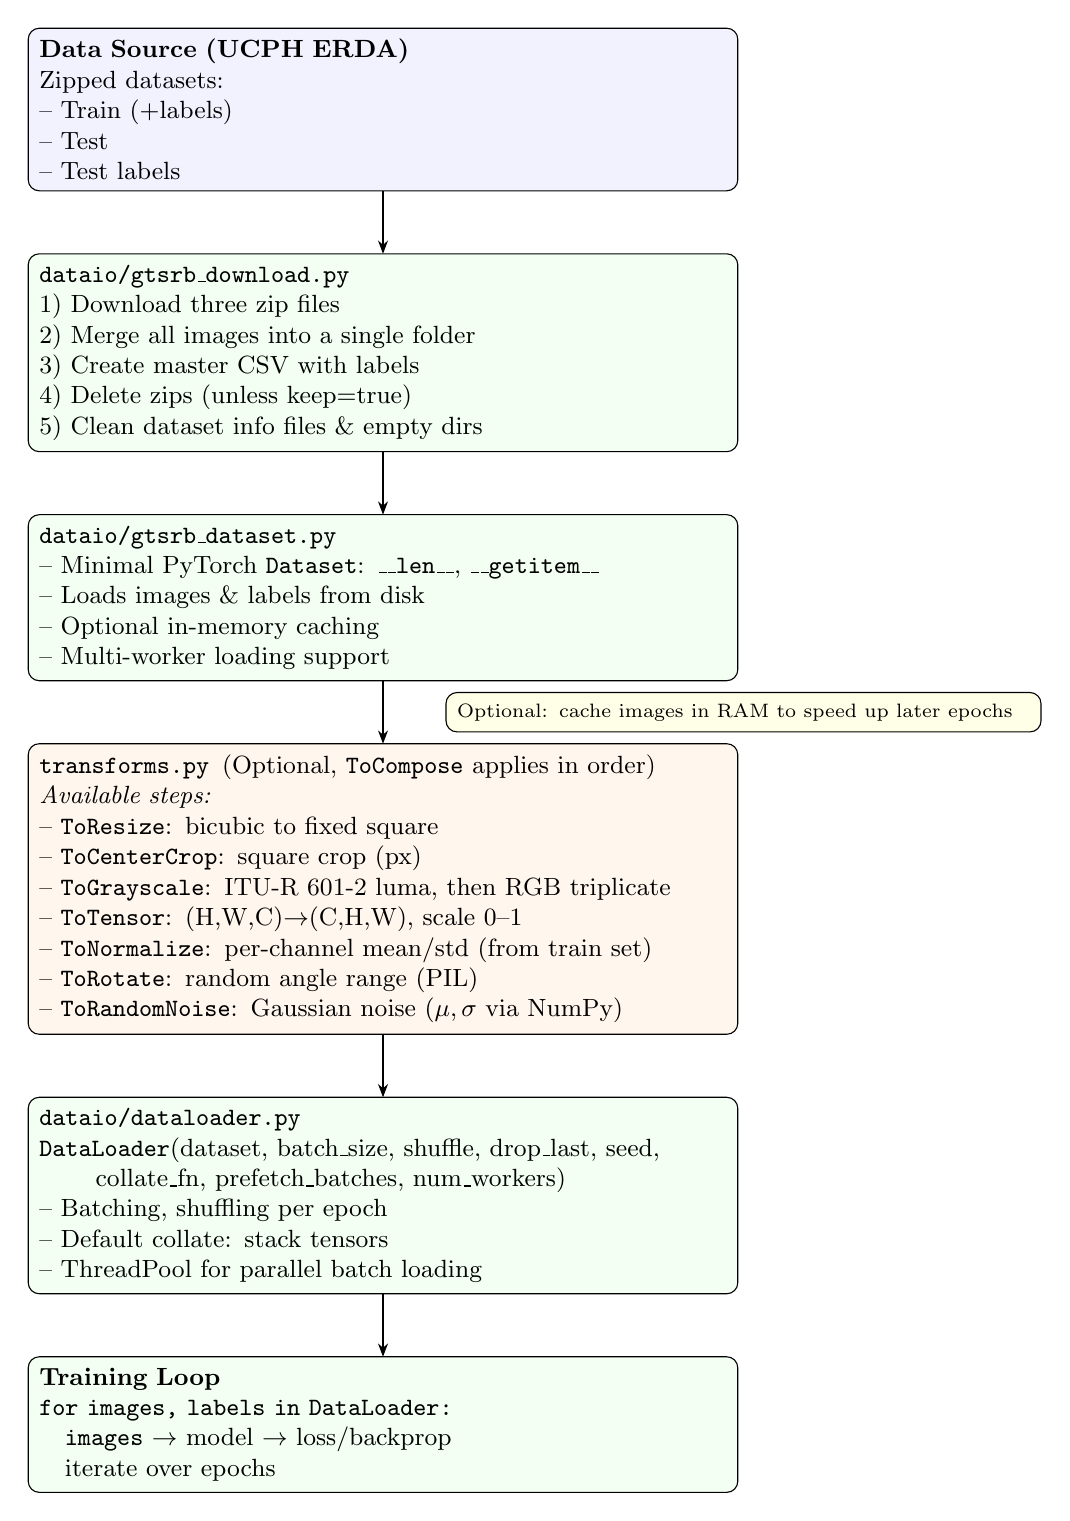
\begin{tikzpicture}[
        node distance=8mm,
        >=Stealth,
        font=\small,
        box/.style={draw, rounded corners, align=left, inner sep=4pt, outer sep=0pt, fill=gray!5},
        io/.style={box, fill=blue!5},
        proc/.style={box, fill=green!5},
        group/.style={box, fill=orange!7},
        note/.style={box, fill=yellow!10, font=\scriptsize},
        every node/.append style={text width=0.72\linewidth}
      ]

      % --- Nodes (stacked vertically to stay narrow) ---
      \node[io] (src) {\textbf{Data Source (UCPH ERDA)}
        \\Zipped datasets:
        \\-- Train (+labels)
        \\-- Test
        \\-- Test labels};

      \node[proc, below=of src] (dl) {\textbf{\texttt{dataio/gtsrb\_download.py}}
      \\1) Download three zip files
      \\2) Merge all images into a single folder
      \\3) Create master CSV with labels
      \\4) Delete zips (unless keep=true)
      \\5) Clean dataset info files \& empty dirs};

      \node[proc, below=of dl] (ds) {\textbf{\texttt{dataio/gtsrb\_dataset.py}}
        \\-- Minimal PyTorch \texttt{Dataset}: \texttt{\_\_len\_\_}, \texttt{\_\_getitem\_\_}
        \\-- Loads images \& labels from disk
        \\-- Optional in-memory caching
        \\-- Multi-worker loading support};

      % Transforms group
      \node[group, below=of ds] (tf) {\textbf{\texttt{transforms.py}} \,(Optional, \texttt{ToCompose} applies in order)
        \\\textit{Available steps:}
        \\-- \texttt{ToResize}: bicubic to fixed square
        \\-- \texttt{ToCenterCrop}: square crop (px)
        \\-- \texttt{ToGrayscale}: ITU-R 601-2 luma, then RGB triplicate
        \\-- \texttt{ToTensor}: (H,W,C)$\to$(C,H,W), scale 0--1
        \\-- \texttt{ToNormalize}: per-channel mean/std (from train set)
        \\-- \texttt{ToRotate}: random angle range (PIL)
        \\-- \texttt{ToRandomNoise}: Gaussian noise (\(\mu,\sigma\) via NumPy)};

      \node[proc, below=of tf] (dlr) {\textbf{\texttt{dataio/dataloader.py}}
        \\\texttt{DataLoader}(dataset, batch\_size, shuffle, drop\_last, seed,
        \\\hspace*{2.2em}collate\_fn, prefetch\_batches, num\_workers)
        \\-- Batching, shuffling per epoch
        \\-- Default collate: stack tensors
        \\-- ThreadPool for parallel batch loading};

      \node[proc, below=of dlr] (train) {\textbf{Training Loop}
        \\\texttt{for images, labels in DataLoader:}
        \\\hspace*{1em}\texttt{images} \(\to\) model \(\to\) loss/backprop
        \\\hspace*{1em}iterate over epochs};

      % --- Arrows ---
      \draw[->] (src) -- (dl);
      \draw[->] (dl) -- (ds);
      \draw[->] (ds) -- node[right, note, xshift=8mm, text width=0.6\linewidth]
      {Optional: cache images in RAM to speed up later epochs} (tf);
      \draw[->] (tf) -- (dlr);
      \draw[->] (dlr) -- (train);

    \end{tikzpicture}%
  }
  \caption{GTSRB data pipeline from download \(\rightarrow\) dataset \(\rightarrow\) transforms \(\rightarrow\) dataloader \(\rightarrow\) training.}
  \label{fig:pipeline}
\end{figure}


\begin{figure}[ht]
  \centering
  \resizebox{\linewidth}{!}{%
    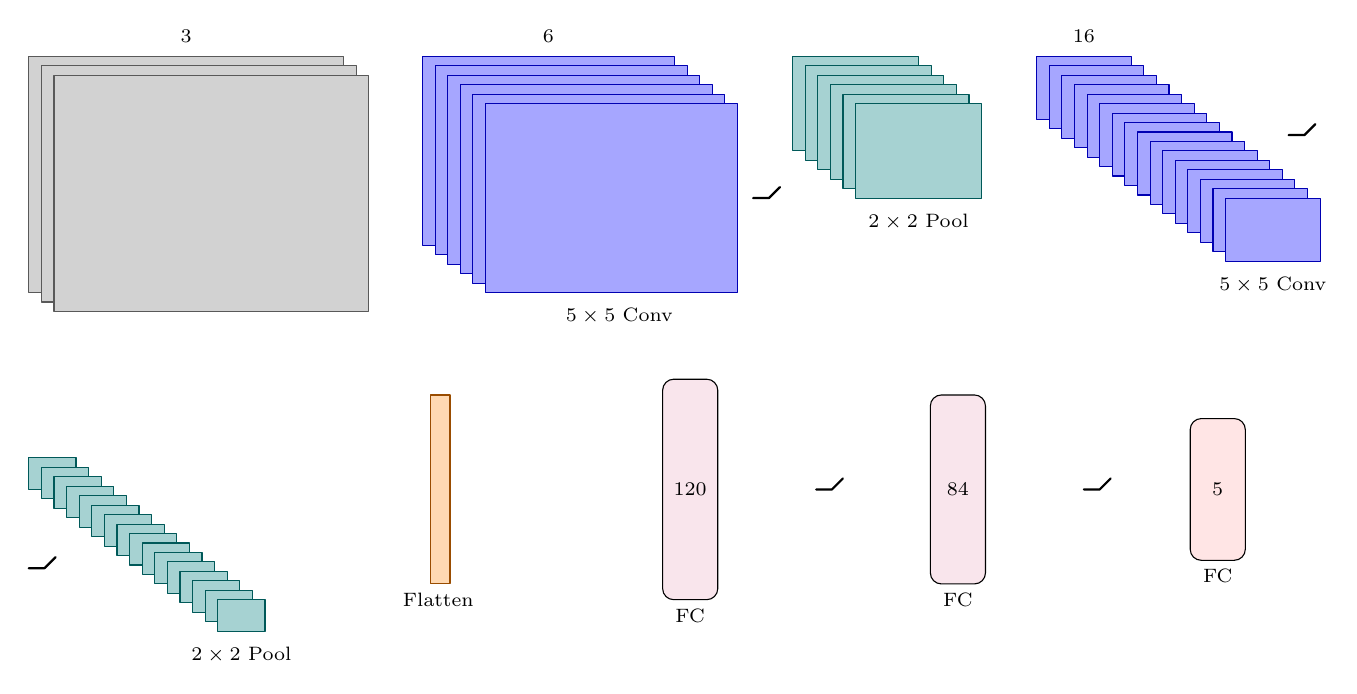
\begin{tikzpicture}[
        >=Stealth, line join=round, line cap=round,
        font=\scriptsize, x=1cm, y=1cm,
        fcbox/.style={draw, rounded corners, minimum width=7mm, minimum height=28mm, fill=purple!10},
        lbl/.style={font=\scriptsize, inner sep=1pt}
      ]
      % ---- helpers ----
      \def\dx{0.16}   % layer stack x-offset
      \def\dy{0.12}   % layer stack y-offset
      \newcommand{\maps}[6]{% x, y, w, h, color, lastIndex
        \begin{scope}[shift={(#1,#2)}]
          \foreach \i in {0,...,#6} {
              \draw[draw=#5!70!black, fill=#5!35] (\i*\dx,-\i*\dy) rectangle ++(#3,#4);
            }
        \end{scope}
      }

      %==================== ROW 1: first four steps ====================
      \def\yA{0} % y for first row

      % 1) Input (3)
      \maps{0}{\yA}{4.0}{3.0}{gray}{2}
      \node[lbl] at (2,\yA+3.25) {$3$};

      % 2) Conv5x5 → 6
      \maps{5}{\yA+0.6}{3.2}{2.4}{blue}{5}
      \node[lbl] at (6.6,\yA+3.25) {$6$};

      % 3) MaxPool2x2
      \maps{9.7}{\yA+1.8}{1.6}{1.2}{teal}{5}

      % 4) Conv5x5 → 16
      \maps{12.8}{\yA+2.2}{1.2}{0.8}{blue}{15}
      \node[lbl] at (13.4,\yA+3.25) {$16$};


      %==================== ROW 2: last five steps =====================
      \def\yB{-2.5} % y for second row (spaced below)
      \def\xStart{0} % left start for second row

      % 5) MaxPool2x2
      \maps{\xStart}{\yB}{0.6}{0.4}{teal}{15}

      % 6) Flatten (thin slab)
      \draw[fill=orange!30, draw=orange!60!black] (\xStart+5.1,\yB-1.2) rectangle ++(0.25,2.4);

      % 7) FC 120
      \node[fcbox] (fc1) at (\xStart+8.4,\yB) {$120$};
      % 8) FC 84
      \node[fcbox, minimum height=24mm] (fc2) at (\xStart+11.8,\yB) {$84$};
      % 9) FC 5 (logits)
      \node[fcbox, minimum height=18mm, fill=red!10] (fc3) at (\xStart+15.1,\yB) {$5$};


      % small ReLU markers (triangles) after convs and FCs
      \foreach \x/\y in {
          9.2/\yA+1.2,
          16/\yA+2,
          \xStart/\yB-1,
          \xStart+10/\yB,
          \xStart+13.4/\yB
        } {
          \draw[black, thick] (\x,\y) -- ++(0.2,0) -- ++(0.14,0.14);
        }

      % labels for minimal cues (kept tiny)
      \node[lbl] at (7.5,\yA-0.3) {$5 \times 5$ Conv};
      \node[lbl] at (11.3,\yA+0.9) {$2 \times 2$ Pool};
      \node[lbl] at (15.8,\yA+0.1) {$5 \times 5$ Conv};
      \node[lbl] at (\xStart+2.7,\yB-2.1) {$2 \times 2$ Pool};
      \node[lbl] at (\xStart+5.2,\yB-1.4) {Flatten};
      \node[lbl] at (\xStart+8.4,\yB-1.6) {FC};
      \node[lbl] at (\xStart+11.8,\yB-1.4) {FC};
      \node[lbl] at (\xStart+15.1,\yB-1.1) {FC};

    \end{tikzpicture}%
  }
  \caption{Visual representation of the original CNN architecture we replicated. The presence of a small ReLU marker indicates a ReLU activation after that layer.}
\end{figure}



\end{document}
